\documentclass[11pt,a4paper]{report}
% Indien je je thesis recto-verso wil afdrukken gebruik je onderstaande opties i.p.v. bovenstaande
%\documentclass[11pt,a4paper,twoside,openright]{report}
\usepackage[a4paper,left=3.5cm, right=2.5cm, top=3.5cm, bottom=3.5cm]{geometry}
\usepackage{graphicx}
\graphicspath{{./figs/}}                        % set graphics path to figs folder, ie now all file imports can be referenced relative to figs
%\usepackage[latin1]{inputenc}                   % om niet ascii karakters rechtstreeks te kunnen inputten
\usepackage[utf8]{inputenc}                    % commentarieer deze regel uit als je utf8 encoded files gebruikt in plaats van latin1
\usepackage[backend=biber, style=ieee, 
citestyle=numeric-comp, maxnames=99]{biblatex}  % make use of the biblatex package to cite references
\addbibresource{bib.bib}
\AtBeginBibliography{\footnotesize}

\usepackage{cmbright}                           % new improved font
\usepackage{listings}             		        % voor het weergeven van broncode
\usepackage[outputdir=cache]{minted}                     % for beautiful listings
\usemintedstyle{borland}
\usepackage{verbatim}					        % weergeven van code, commando's, ...
\usepackage{hyperref}					        % maak PDF van de thesis navigeerbaar
\usepackage{url}						        % URL's invoegen in tekst met behulp van \url{http://}
\usepackage[small,bf,hang]{caption}             % om de captions wat te verbeteren
\usepackage[final]{pdfpages}                    % gebruikt voor het invoegen van het artikel in pdf-formaat
%\usepackage{pslatex}					        % andere lettertype's dan de standaard types

%\usepackage{sectsty}					        % aanpassen van de fonts van sections en chapters
%\allsectionsfont{\sffamily}
%\chapterfont{\raggedleft\sffamily}

\usepackage{float}                              % De optie H voor de plaatsing van figuren op de plaats waar je ze invoegt. bvb. \begin{figure}[H]
%\usepackage{longtable}					        % tabellen die over meerdere pagina's gespreid worden
%\usepackage[times]{quotchap}                   % indien je fancy hoofdstuktitels wil
%\usepackage[none]{hyphenat}
%\usepackage{latexsym}
\usepackage{amsmath}
\usepackage{amssymb}
\usepackage{siunitx}
\sisetup{detect-all}
\usepackage[acronym,xindy]{glossaries}
\makenoidxglossaries
\usepackage[version=4]{mhchem}                  % chemical formulas
\usepackage{tabularx}
\usepackage{booktabs}                           % nice tables
\usepackage{array}                              % fixed-width columns in tables

%%%% Tikz %%%%
\usepackage{pgfplots}
\DeclareUnicodeCharacter{2212}{−}
\usepgfplotslibrary{groupplots,dateplot}
\usetikzlibrary{patterns,shapes.arrows}
\pgfplotsset{compat=newest}
%%%%%%%%%%%% MAKE FIGURES MORE UNIFORM %%%%%%%%%%%%
\definecolor{darkgray176}{RGB}{176,176,176}
\definecolor{color0}{RGB}{255,127,14}
\definecolor{color1}{RGB}{44,160,44}
\pgfplotsset{
    every axis/.append  style={
        title style={draw=none},
        label style={font=\small},
        legend style={
            fill opacity=0.8,
            nodes={scale=0.8, transform shape}, {draw=none}
        },
        tick align=outside,
        tick pos=left,
        x grid style={darkgray176},
        xtick style={color=black},
        y grid style={darkgray176},
        ytick style={color=black},
        grid=both,
    },
    every axis plot/.append style={
        line width=1.0pt,
        mark size=1,
    },
}


% used commands
\usepackage{xspace}
\usepackage{idpz3syntax}
\usepackage{decision-table}
\newcommand{\fodot}{FO($\cdot$)\xspace}

%%%%%%%%%%%% choose your campus and language %%%%%%%%%%%%
\usepackage{fiiw} 



%door onderstaande regels in commentaar te zetten, of op false, kan je pagina's weglaten
%bijvoorbeeld het weglaten van een voorwoord, lijst met symbolen, ...
%%%%%%%%%%%%%%%%%%%%%%%%%%%%%%%%%%%%%%%%%%%%%%%%%%%%%%%%%%%%%%%%%%%%%%%%%%%%%%%%%%%%%%%%
%voorwoord toevoegen?
%\acknowledgementspagetrue
%\acknowledgements{voorwoord}			%.tex file met daarin het voorwoord
%abstract toevoegen?
%\abstractpagetrue
%\abstracts{abstract}					%.tex file met daarin het abstract
%lijst van figuren toevoegen?
%\listoffigurespagetrue
%lijst van tabellen toevoegen?
%\listoftablespagetrue
%lijst van symbolen toevoegen?
%\listofsymbolspagetrue
%\listofsymbols{symbolen}				%.tex file met daarin de lijst van symbolen


% Information about your discipline
%%%%%%%%%%%%%%%%%%%%%%%%%%%%%%%%%%%%%%%%%%%%%%%

\opleiding{Electronica-ICT}
%\afdeling{Software Engineer}
\campus{denayereng}                       % Define your campus and language (append "eng" to load the English template)
                                            % campuses: denayer, geel, gent, groept, brugge (denayereng, geeleng, ghenteng, groupteng, brugeseng)
\title{User-friendly House\\ Automation using IDP}
\subtitle{}
\forenameA{Thijs}
\surnameA{Alens}
\forenameB{} %keep empty if no 2nd author
\surnameB{} %keep empty if no 2nd author
\academicyear{2024 - 2025}

% NOG PROBLEMEN MET VOORBLAD -> fiiw.sty lijn ~326
  

\promotorA[Supervisor(s)]{S. Vandevelde} %for English use Supervisor(s)
\promotorB[Assistant supervisor(s)]{L. Van Laer}

% generated by Gilles Callebaut with the script: https://github.com/DRAMCO/writing-scientific-papers-in-latex-tips-and-tricks/blob/main/glossaries/merge_abbr.py

%%%%%%%%%%%% 2 %%%%%%%%%%%%
\newacronym{2d}{2D}{two-dimensional}
%%%%%%%%%%%% 3 %%%%%%%%%%%%
\newacronym{3d}{3D}{three-dimensional}
\newacronym{3gpp}{3GPP}{3rd generation partnership project}
%%%%%%%%%%%% 5 %%%%%%%%%%%%
\newacronym{5g}{5G}{fifth-generation}
%%%%%%%%%%%% 6 %%%%%%%%%%%%
\newacronym{6g}{6G}{sixth-generation}
%%%%%%%%%%%% A %%%%%%%%%%%%
\newacronym{abp}{ABP}{authentication by personalisation}
\newacronym{aclr}{ACLR}{adjacent channel leakage ratio}
\newacronym{adc}{ADC}{Analog-to-digital converter}
\newacronym{adr}{ADR}{adaptive data rate}
\newacronym{ag}{AG}{array gain}
\newacronym{ai}{AI}{artificial intelligence}
\newacronym{amam}{AM/AM}{amplitude modulation to amplitude modulation}
\newacronym{amp}{AMP}{approximate message passing}
\newacronym{ampm}{AM/PM}{amplitude modulation to phase modulation}
\newacronym{aoa}{AOA}{angle-of-arrival}
\newacronym{aod}{AOD}{angle-of-departure}
\newacronym{ap}{AP}{access point}
\newacronym{apu}{APU}{access point unit}
\newacronym{ar}{AR}{augmented reality}
\newacronym{arp}{ARP}{Antenna Reference Point}
\newacronym{asic}{ASIC}{application specific integrated circuit}
\newacronym{ask}{ASK}{amplitude-shift keying}
\newacronym{auv}{AUV}{autonomous underwater vehicle}
\newacronym{awgn}{AWGN}{additive white Gaussian noise}
%%%%%%%%%%%% B %%%%%%%%%%%%
\newacronym{baw}{BAW}{bulk acoustic wave}
\newacronym{bb}{BB}{base-band}
\newacronym{bf}{BF}{beamforming}
\newacronym{bldc}{BLDC}{brushless DC}
\newacronym{bom}{BOM}{bill of materials}
\newacronym{bs}{BS}{base station}
\newacronym{bw}{BW}{bandwidth}
%%%%%%%%%%%% C %%%%%%%%%%%%
\newacronym{cad}{CAD}{channel activity detection}
\newacronym{cars}{CARS}{calibration reference signal}
\newacronym{cbm}{CBM}{condition based maintenance}
\newacronym{cc}{CC}{constant current}
\newacronym{ccdf}{CCDF}{complementary cumulative distribution function}
\newacronym{ccnn}{CCNN}{circular convolutional neural network}
\newacronym{ccs}{CCS}{correlative channel sounder}
\newacronym{cdf}{CDF}{cumulative distribution function}
\newacronym{cdrx}{CDRX}{connected mode DRX}
\newacronym{ce}{CE}{coverage enhancement}
\newacronym{ced}{CED}{cumulative energy density}
\newacronym{cf}{CF}{cell-free}
\newacronym{cfo}{CFO}{carrier frequency offset}
\newacronym{cir}{CIR}{channel impulse response}
\newacronym{cost}{COST}{commercial off-the-shelf}
\newacronym{cots}{COTS}{commercial off-the-shelf}
\newacronym{cp}{CP}{cyclic prefix}
\newacronym{cpt}{CPT}{capacitive power transfer}
\newacronym{cpu}{CPU}{central-processing unit}
\newacronym{cqi}{CQI}{channel quality indicator}
\newacronym{cr}{CR}{coding rate}
\newacronym{crlb}{CRLB}{Cram\'er-Rao lower bound}
\newacronym{crs}{CRS}{cell reference signal}
\newacronym{cs}{CS}{compressed sensing}
\newacronym{csi}{CSI}{channel state information}
\newacronym{csp}{CSP}{contact service point}
\newacronym{css}{CSS}{chirp spread spectrum}
\newacronym{cv}{CV}{constant voltage}
%%%%%%%%%%%% D %%%%%%%%%%%%
\newacronym{dac}{DAC}{digital-to-analog converter}
\newacronym{daq}{DAQ}{data acquisition system}
\newacronym{dc}{DC}{direct current}
\newacronym{dcc}{DCC}{dynamic cooperation clustering}
\newacronym{de}{DE}{drain efficiency}
\newacronym{dl}{DL}{downlink}
\newacronym{dlc}{DLC}{Distributed Laser Charging}
\newacronym{dma}{DMA}{Direct Memory Access}
\newacronym{dmimo}{D-MIMO}{distributed MIMO}
\newacronym{dpd}{DPD}{digital pre-distortion}
\newacronym{dpdk}{DPDK}{Data Plane Development Kit}
\newacronym{drx}{DRX}{Discontinuous Reception Mode}
\newacronym{duc}{DUC}{digital up-converter}
%%%%%%%%%%%% E %%%%%%%%%%%%
\newacronym{e2e}{E2E}{end-to-end}
\newacronym{easa}{EASA}{European Union Aviation Safety Agency}
\newacronym{ecdf}{eCDF}{empirical cumulative distribution function}
\newacronym{ecsp}{ECSP}{edge computing service point}
\newacronym{edlc}{EDLC}{electrostatic double-layer capacitors}
\newacronym{edrx}{eDRX}{Extended Discontinuous Reception Mode}
\newacronym{ee}{EE}{energy efficiency}
\newacronym{egprs}{EGPRS}{Enhanced Data Rates for GSM Evolution}
\newacronym{eirp}{EIRP}{effective isotropic radiated power}
\newacronym{em}{EM}{electromagnetic}
\newacronym{embb}{eMBB}{enhanced Mobile Broadband}
\newacronym{en}{EN}{energy neutral}
\newacronym{eol}{EoL}{end of life}
\newacronym{epu}{EPU}{edge processing unit}
\newacronym{erp}{ERP}{effective radiated power}
\newacronym[plural=ESCs,firstplural=electronic speed controllers (ESCs)]{esc}{ESC}{electronic speed control}
\newacronym{etsi}{ETSI}{European Telecommunications Standards Institute}
\newacronym{evm}{EVM}{Error Vector Magnitude}
%%%%%%%%%%%% F %%%%%%%%%%%%
\newacronym{fa}{FA}{federation anchor}
\newacronym{fembb}{feMBB}{further enhanced mobile broadband}
\newacronym{fft}{FFT}{fast Fourier transform}
\newacronym{fh}{FH}{fronthaul}
\newacronym{fim}{FIM}{Fisher information matrix}
\newacronym{fom}{FoM}{figure of merit}
\newacronym{fpga}{FPGA}{field-programmable gate array}
%%%%%%%%%%%% G %%%%%%%%%%%%
\newacronym{gb}{GB}{grant-based}
\newacronym{gf}{GF}{grant-free}
\newacronym{gnb}{gNB}{Next Generation Node B}
\newacronym{gnn}{GNN}{graph neural network}
\newacronym{gnss}{GNSS}{global navigation satellite system}
\newacronym{gpclk}{GPCLK}{general purpose clock}
\newacronym{gprs}{GPRS}{General Packet Radio Services}
\newacronym{gps}{GPS}{Global Positioning System}
\newacronym{gpu}{GPU}{graphical processing unit}
\newacronym{gsm}{GSM}{Global System for Mobile Communications}
\newacronym{gwp}{GWP}{Global Warming Potential}
%%%%%%%%%%%% H %%%%%%%%%%%%
\newacronym{harq}{HARQ}{hybrid automatic repeat request}
\newacronym{hat}{HAT}{hardware attached on top}
\newacronym{hcs}{HCS}{human-centric services}
\newacronym{hpbm}{HPBM}{half power beam width}
%%%%%%%%%%%% H %%%%%%%%%%%%
\newacronym{HyMPRo}{HyMPRo}{Hybrid Multi-Path Routing algorithm}
%%%%%%%%%%%% I %%%%%%%%%%%%
\newacronym{ib}{IB}{in-band}
\newacronym{ibo}{IBO}{input back-off}
\newacronym{ic}{IC}{integrated circuit}
\newacronym{id}{ID}{information decoding}
\newacronym{if}{IF}{intermediate-frequency}
\newacronym{iid}{i.i.d.}{independently and identically distributed}
\newacronym{im}{IM}{intermodulation}
\newacronym{imu}{IMU}{inertial measurement unit}
\newacronym{io}{IO}{input/output}
\newacronym{iot}{IoT}{Internet of Things}
\newacronym{ipt}{IPT}{inductive power transfer}
\newacronym{ipy}{IPY}{Interventions per Year}
\newacronym{iq}{IQ}{in-phase and quadrature}
\newacronym{ir}{IR}{infrared}
\newacronym{ism}{ISM}{industrial, scientific and medical}
\newacronym{isp}{ISP}{internet service provider}
%%%%%%%%%%%% K %%%%%%%%%%%%
\newacronym{kpi}{KPI}{key performance indicator}
\newacronym{kvi}{KVI}{key value indicator}
%%%%%%%%%%%% L %%%%%%%%%%%%
\newacronym{lca}{LCA}{life cycle assessment}
\newacronym{lco}{LCO}{lithium cobalt oxide}
\newacronym{ldo}{LDO}{Low-dropout voltage regulator}
\newacronym{ldpc}{LDPC}{low-density parity-check}
\newacronym{lfp}{LFP}{lithium iron phosphate}
\newacronym{lic}{LIC}{lithium-ion capacitor}
\newacronym{lidar}{LiDAR}{light detection and ranging}
\newacronym{liion}{Li-ion}{lithium-ion}
\newacronym{lipo}{LiPo}{lithium polymer}
\newacronym{lis}{LIS}{large intelligent surface}
\newacronym{llh}{LLH}{log-likelihood}
\newacronym{lmmse}{LMMSE}{least minimum mean square error}
\newacronym{lmo}{LMO}{lithium ion manganese oxide}
\newacronym{lo}{LO}{local oscillator}
\newacronym{lora}{LoRa}{long range}
\newacronym{lorawan}{LoRaWAN}{long-range wide-area network}
\newacronym{los}{LoS}{line-of-sight}
\newacronym{lp}{LP}{linear programming}
\newacronym{lpt}{LPT}{laser power transfer}
\newacronym{lpwa}{LPWA}{Low Power Wide Area}
\newacronym{lpwan}{LPWAN}{low-power wide-area network}
\newacronym{lqi}{LQI}{link quality indicator}
\newacronym{lrelu}{LReLU}{leaky rectified linear unit}
\newacronym{lrt}{LRT}{likelihood-ratio test}
\newacronym{ls}{LS}{least squares}
\newacronym{lsa}{LSA}{large synthetic array}
\newacronym{lsfc}{LSFC}{large-scale fading component}
\newacronym{ltc}{LTC}{lithium thionyl chloride}
\newacronym{lte}{LTE}{Long Term Evolution}
\newacronym{lto}{LTO}{lithium titanate}
%%%%%%%%%%%% M %%%%%%%%%%%%
\newacronym{m2m}{M2M}{machine to machine}
\newacronym{mac}{MAC}{Medium Access Control}
\newacronym{mate}{MATE}{millimeter-wave MIMO testbed}
\newacronym{mcl}{MCL}{Maximum Coupling Loss}
\newacronym{mcs}{MCS}{modulation and coding scheme}
\newacronym{mcu}{MCU}{Microcontroller Unit}
\newacronym{mec}{MEC}{multi-access edge computing}
\newacronym{mems}{MEMS}{micro-electromechanical systems}
\newacronym{mf}{MF}{matched filter}
\newacronym{mimo}{MIMO}{multiple-input multiple-output}
\newacronym{miso}{MISO}{multiple-input single-output}
\newacronym{ml}{ML}{machine learning}
\newacronym{mlp}{MLP}{multilayer perceptron}
\newacronym{mmimo}{mMIMO}{massive MIMO}
\newacronym{mmse}{MMSE}{minimum mean square error}
\newacronym{mmtc}{mMTC}{massive machine-typed communication}
\newacronym{mmwave}{mmWave}{millimeter wave}
\newacronym{mpc}{MPC}{multipath component}
\newacronym{mppt}{MPPT}{maximum power point tracking}
\newacronym{mr}{MR}{maximum ratio}
\newacronym{mrc}{MRC}{maximum ratio combining}
\newacronym{mrc_em}{MRC}{maximum ratio combining}
\newacronym{mrc_EM}{MRC}{Magnetic Resonance Coupling}
\newacronym{mrt}{MRT}{maximum ratio transmission}
\newacronym{mse}{MSE}{mean square error}
\newacronym{mtc}{MTC}{Machine-Type Communication}
\newacronym{multi-rat}{Multi-RAT}{multiple radio access technology}
%%%%%%%%%%%% N %%%%%%%%%%%%
\newacronym{nb}{NB}{narrowband}
\newacronym{nbiot}{NB-IoT}{narrowband IoT}
\newacronym{nca}{NCA}{nickel cobalt aluminum}
\newacronym{nicd}{NiCd}{nikkel cadmium}
\newacronym{nimh}{NiMH}{nikkel metal hydride}
\newacronym{nlos}{NLoS}{non-line-of-sight}
\newacronym{nmc}{NMC}{nickel manganese cobalt}
\newacronym{nn}{NN}{neural network}
\newacronym{nnls}{NNLS}{non-negative least squares}
\newacronym{noma}{NOMA}{non-orthogonal multiple access}
\newacronym{nr}{NR}{New Radio}
\newacronym{ntp}{NTP}{network time protocol}
%%%%%%%%%%%% O %%%%%%%%%%%%
\newacronym{oai}{OAI}{OpenAirInterface} % no spelling mistake, it is spelled all glued to eachother...
\newacronym{ofdm}{OFDM}{orthogonal frequency-division multiplexing}
\newacronym{ofdmim}{OFDM-IM}{OFDM with index modulation}
\newacronym{oob}{OOB}{out-of-band}
\newacronym{oran}{O-RAN}{open radio-access network}
\newacronym{os}{OS}{operating system}
\newacronym{ota}{OTA}{over-the-air}
\newacronym{otaa}{OTAA}{over-the-air authentication}
%%%%%%%%%%%% P %%%%%%%%%%%%
\newacronym{p2p}{P2P}{point-to-point}
\newacronym{pa}{PA}{power amplifier}
\newacronym{pae}{PAE}{power-added efficiency}
\newacronym{papr}{PAPR}{peak-to-average power ratio}
\newacronym{pc}{PC}{pilot count}
\newacronym{pcb}{PCB}{printed circuit board}
\newacronym{pcg}{PCG}{power consumption gain}
\newacronym{pd}{PD}{powered device}
\newacronym{pdcch}{PDCCH}{physical downlink control channel}
\newacronym{pdp}{PDP}{power delay profile}
\newacronym{pdsch}{PDSCH}{physical downlink shared channel}
\newacronym{per}{PER}{packet error rate}
\newacronym{pg}{PG}{path gain}
\newacronym{pgd}{PGD}{proximal gradient descent}
\newacronym{pl}{PL}{path loss}
\newacronym{pll}{PLL}{phase-locked loop}
\newacronym{poe}{PoE}{power-over-Ethernet}
\newacronym{pps}{1PPS}{pulse per second}
\newacronym{prbs}{PRBs}{Physical Resource Blocks}
\newacronym{ps}{PS}{Processing System}
\newacronym{psd}{PSD}{power spectral density}
\newacronym{pse}{PSE}{power sourcing equipment}
\newacronym{psm}{PSM}{power saving mode}
\newacronym{pss}{PSS}{primary synchronisation signal}
\newacronym{ptp}{PTP}{precision-time protocol}
\newacronym{ptrs}{PTRS}{Phase-Tracking Reference Signals}
\newacronym{ptw}{PTW}{paging time window}
\newacronym{pwm}{PWM}{pulse width modulation}
%%%%%%%%%%%% Q %%%%%%%%%%%%
\newacronym{qam}{QAM}{quadrature amplitude modulation}
\newacronym{qos}{QoS}{quality-of-service}
\newacronym{quadriga}{QuaDRiGa}{QUAsi Deterministic RadIo channel GenerAtor}
%%%%%%%%%%%% R %%%%%%%%%%%%
\newacronym{ra}{RA}{Random Access}
\newacronym{ran}{RAN}{radio access network}
\newacronym{rar}{RAR}{Random Access Response}
\newacronym{rat}{RAT}{radio access technology}
\newacronym{rbs}{RBS}{radio base station}
\newacronym{re}{RE}{radio element}
\newacronym[]{relu}{ReLU}{rectified linear unit}
\newacronym{rf}{RF}{radio frequency}
\newacronym{rfeh}{RFEH}{radio frequency energy harvesting}
\newacronym{rfic}{RFIC}{radio-frequency integrated circuit}
\newacronym{rfid}{RFID}{radio frequency identification}
\newacronym{rfpt}{RFPT}{radio frequency power transfer}
\newacronym{rfsoc}{RFSoC}{Radio Frequency System-on-Chip}
\newacronym{ris}{RIS}{reflective intelligent surface}%reconfigurable?
\newacronym{rllmtc}{RLLMTC}{reliable low latency machine type communication}
\newacronym{rms}{RMS}{root-mean-square}
\newacronym{rmse}{RMSE}{root-mean-square error}
\newacronym{rof}{RoF}{radio-over-fiber}
\newacronym{ros}{ROS}{robot operating system}
\newacronym{rpi}{RPi}{Raspberry Pi}
\newacronym{rrc}{RRC}{Radio Resource Connection}
\newacronym{rreq}{RREQ}{route request packet}
\newacronym{rsrp}{RSRP}{Reference Signals Received Power}
\newacronym{rss}{RSS}{received signal strength}
\newacronym{rssi}{RSSI}{received signal strength indicator}
\newacronym{rtc}{RTC}{real time clock}
\newacronym{rtk}{RTK}{real time kinematics}
\newacronym{rts}{RTS}{ray tracing simulator}
\newacronym{rw}{RW}{RadioWeaves}
\newacronym{rx}{RX}{receiver}
\newacronym{rzf}{RZF}{regularized zero forcing}
%%%%%%%%%%%% S %%%%%%%%%%%%
\newacronym{sa}{SA}{synchronization anchor}
\newacronym{scfdma}{SCFDMA}{single-carrier frequency division multiple access}
\newacronym{sdg}{SDG}{Sustainable Development Goal}
\newacronym{sdm}{SDM}{sigma-delta modulator}
\newacronym{sdn}{SDN}{software-defined network}
\newacronym{sdof}{SDoF}{sigma-delta over fiber}
\newacronym{sdr}{SDR}{software-defined radio}
\newacronym{sf}{SF}{spreading factor}
\newacronym{sfn}{SFN}{single frequency network}
\newacronym{sfp}{SFP}{small form-factor pluggable}
\newacronym{sinr}{SINR}{signal-to-interference-plus-noise ratio}
\newacronym{siso}{SISO}{single-input single-output}
\newacronym{slam}{SLAM}{simultaneous localization and mapping}
\newacronym{slc}{SLC}{spatial leakage suppression}
\newacronym{smc}{SMC}{specular multipath component}
\newacronym{smps}{SMPS}{switched mode power supply}
\newacronym{sndr}{SNDR}{signal-to-noise-and-distortion ratio}
\newacronym{snidr}{SNIDR}{signal-to-noise-and-interference-and-distortion ratio}
\newacronym{snr}{SNR}{signal-to-noise ratio}
\newacronym{soc}{SoC}{state of charge}
\newacronym{ssb}{SSB}{synchronisation signal block}
\newacronym{ssd}{SSD}{solid state drive}
\newacronym{steam}{STEAM}{science, technology, engineering, the arts, and mathematics}
\newacronym{svd}{SVD}{singular value decomposition}
%%%%%%%%%%%% T %%%%%%%%%%%%
\newacronym{tau}{TAU}{tracking area update}
\newacronym{tcer}{TCER}{transported to consumed energy ratio}
\newacronym{tdd}{TDD}{time division duplexing}
\newacronym{tdoa}{TDOA}{time-difference-of-arrival}
\newacronym{toa}{TOA}{time-of-arrival}
\newacronym{tof}{ToF}{time-of-flight}
\newacronym{tosm}{TOSM}{through-open-short-match}
\newacronym{trl}{TRL}{technology readyness level}
\newacronym{trp}{TRP}{Transmission Reception Point}
\newacronym{tsn}{TSN}{time-sensitive networking}
\newacronym{ttm}{TTM}{time to market}
\newacronym{ttn}{TTN}{The Things Network}
\newacronym{tx}{TX}{transmitter}
%%%%%%%%%%%% U %%%%%%%%%%%%
\newacronym{uav}{UAV}{unmanned aerial vehicle}
\newacronym{udp}{UDP}{User Datagram Protocol}
\newacronym{ue}{UE}{user equipment}
\newacronym{ugv}{UGV}{unmanned ground vehicle}
\newacronym{uhd}{UHD}{USRP hardware driver}
\newacronym{uhf}{UHF}{ultra-high frequency}
\newacronym{ul}{UL}{uplink}
\newacronym{ula}{ULA}{uniform linear array}
\newacronym{ummtc}{umMTC}{ultra massive machine type communication}
\newacronym{upa}{UPA}{uniform planar array}
\newacronym{ura}{URA}{uniform rectangular array}
\newacronym{urllc}{URLLC}{ultra-reliable low-latency communications}
\newacronym{usrp}{USRP}{universal software radio peripheral}
\newacronym{uv}{UV}{unmanned vehicle}
\newacronym{uwb}{UWB}{ultrawideband}
%%%%%%%%%%%% V %%%%%%%%%%%%
\newacronym{vep}{VEP}{virtual edge platform}
\newacronym{vlc}{VLC}{visible light communication}
\newacronym{vlp}{VLP}{visible light positioning}
\newacronym{vna}{VNA}{vector network analyzer}
\newacronym{vr}{VR}{virtual reality}
%%%%%%%%%%%% W %%%%%%%%%%%%
\newacronym{wb}{WB}{wideband}
\newacronym{wpt}{WPT}{wireless power transfer}
\newacronym{wr}{WR}{White Rabbit}
\newacronym{wrsn}{WRSN}{wireless rechargeable sensor network}
\newacronym{wsn}{WSN}{wireless sensor network}
%%%%%%%%%%%% X %%%%%%%%%%%%
\newacronym{xr}{XR}{extended reality}
%%%%%%%%%%%% Z %%%%%%%%%%%%
\newacronym{z3ro}{Z3RO}{zero third-order distortion}
\newacronym{zf}{ZF}{zero-forcing}
\newacronym{zmcscg}{ZMCSCG}{zero mean circularly symmetric complex Gaussian}


\begin{document}
\preface%

\printnoidxglossary[type=\acronymtype]%
\clearpage

%\input{hfdst1}
%\input{hfdst2}
%\input{hfdst3}


% Eventueel enkele appendices
%%%%%%%%%%%%%%%%%%%%%%%%%%%%%%


% Bijlage met daarin het wetenschappelijk artikel
%%%%%%%%%%%%%%%%%%%%%%%%%%%%%%%%%%%%%%%%%%%%%%%%%%
%\chapter{Beschrijving van deze masterproef in de vorm van een wetenschappelijk artikel}
%The thesis should also contain a short scientific article. If you write your thesis in Dutch, you must write the article in English, and vice versa. We advise you to employ the IEEE Manuscript Templates for Conference Proceedings (\url{https://www.overleaf.com/latex/templates/ieee-conference-template/grfzhhncsfqn}).

\chapter{Introduction}
\section{Positioning}
We are living in a world where automation is increasing rapidly. From automatically sorting luggage to the right plane at the airport, to fully self-driving cars, automation is becoming an integral part of our lives. This evolution, paired with the emergence of the Internet of Things (IoT), where many devices have become ``smart'' and automation-ready, has not only revolutionized industries but also opened up new possibilities for homeowners.

In essence, home automation is a way to automate tasks in a home. These can be simple tasks such as automatically turning on lights upon entering a room, to more advanced operations like regulating home climate. This has the potential to significantly streamline daily routines, reduce costs, and improve overall comfort.

One way to configure a home environment is by using a home automation system that runs on a local server in conjunction with Home Assistant (HA). HA is an application that integrates various devices from different brands into a single functional app. It also provides a framework through which users can automate their homes.

A home automation system is essentially a set of rules that define the behavior of the home, making it well-suited for a knowledge-based system. Such a system requires the user to input a set of rules, which are then processed by a reasoning engine to make the necessary decisions.

IDP-Z3 is an example of such a reasoning engine, utilizing a formal description to define these rules. One of the key advantages of IDP-Z3 is its ability to separate knowledge from its application. This separation allows users to focus on defining the rules without needing to program the decision-making process themselves, as the reasoning engine handles this automatically.

\section{Problem statement}
One of the main challenges is the steep learning curve associated with setting up and maintaining home automation systems. If users wish to implement their own home automation, they can use home assistants's user interface (UI). Automations, however, require that the user has a basic understanding of programming and is familiar with specific technical tools. This way they can manually modify the configuration files and troubleshoot any issues that may be presented, which is not easily done by non-experts.

IDP-Z3 can make this process simpler by making use of a declarative knowledge base, avoiding the need to program automations. However, the IDP-Z3 language itself is not particularly user-friendly for non-experts and can become quite complex, especially when dealing with intricate rules or scenarios. When users are confronted with a large problem domain, it can be difficult to maintain an overview and make necessary adjustments. It also has a lot of possibilities that are not useful in the context of home automation, which can be confusing or overwelming.

\section{Objectives}
This thesis seeks to address this issue by investigating how IDP, specifically IDP-Z3, can be utilized to make home automation more accessible. Instead of needing to create automations, triggers, and aligning them with each other, the user only needs to describe the desired behavior of the home in a declarative language. A graphical user interface (GUI) that provides structure, along with a more limited subset of the IDP language, could help make IDP a more viable option for home automation.\\
The primary research question addressed in this thesis is:\\
How do we design an IDP-Z3 framework that enables end-users to automate their homes in a user-friendly way?\\
This overarching question is further explored through the following sub-questions:
\begin{itemize}
    \item What is the optimal user-friendly interface for addressing this problem?
    \item Which subset of the IDP-language is needed to configure a home?
\end{itemize}
The objectives of this thesis are:
\begin{itemize}
    \item Decide on a subset of the IDP-language that has all the functionality needed for home automation.
    \item Design a user-friendly UI that is most suited for IDP in combination with home automation.
\end{itemize}





\chapter{Literature review}
In this chapter, we discuss existing research relevant to the topics covered in this thesis. First, we elaborate on home automation, with a brief overview of HA and how users can configure their homes using it. Next, we will explore the basics of \fodot and IDP-Z3. After that, we will examine existing user-friendly \fodot alternatives, highlighting their strengths and weaknesses in the context of this use case. To close we will discuss the state of the art and how we can learn from it.
\section{Home automation}
Home automation is a broad term used when discussing the automation of a home. It ranges from simple tasks, such as automatically turning on a light when entering a room, to complex tasks, like adjusting the house temperature based on various variables. It also refers to home security: when should the security camera automatically record, when should the doors automatically lock, what should happen if the alarm goes off, etc. Automating tasks, like automatically making coffee at the start of the day, is also considered part of home automation. Additionally, it can help manage energy consumption throughout the day to reduce costs.

Home automation consists of 3 main parts:
\begin{itemize}
    \item Smart home devices
    \item A smart hub/server
    \item An application
\end{itemize}

\paragraph{Smart home devices}
A smart home device (or smart device) can be either of two things: a sensor or an actuator. A sensor can detect an event, while an actuator can respond to a trigger. A simple example is a motion detector (sensor) that automatically turns on a light (actuator) when there is movement (trigger). Depending on the device, there may be some additional (smart) features. For example, the light could have an internal clock that provides the current time. This allows the light to automatically adjust its brightness based on the expected amount of natural light at that time. In summary, smart devices are the physical hardware (sensors and actuators) combined with software used for the communication between devices, which, in most cases, do not contain any smart home logic themselves.

\paragraph{Smart hub/server}
The smart hub is a central device that connects the complex hardware of smart devices to the user. Its function is to receive data from sensors and send commands to actuators, serving as a central hub for the devices, so to speak. This hub can be provided by a manufacturer specifically for their smart devices, or it can be a generic one designed to be compatible with as many devices as possible.

\paragraph{Application}
The application allows the user to configure their home. Most often, this is done through a graphical user interface (GUI) where the user can create automations, view the status of devices, monitor active automations, easily communicate with the devices, etc.

\subsection{Home assistant}
\label{HomeAssistant}

Home assistant (HA)~\cite{HA} is an open-source, all-in-one application for home automation. In a home environment, it typically  runs on a local server, where smart devices can be connected and configured. Because it is local, it provides strong security for user data. HA has a large and growing community, which ensures compatibility with a wide range of devices and brands, eliminating the need for multiple apps to control a home environment.\\
HA also offers multiple UIs (known as dashboards) where users can monitor the state of their home. Users can select a dashboard created by others, design one themselves, or build on an existing dashboard. They can interact with their devices directly through these dashboards. Additionally, users can create automations using a separate UI, which are actions executed when a set trigger occurs. Fully understanding how these automations work requires a deeper understanding of how HA functions.
In the following paragraphs we will discuss some terminology used inside HA. 
An overview of these concepts is shown in Figure~\ref{fig:ha_structure}.

\begin{figure}
    \centering
    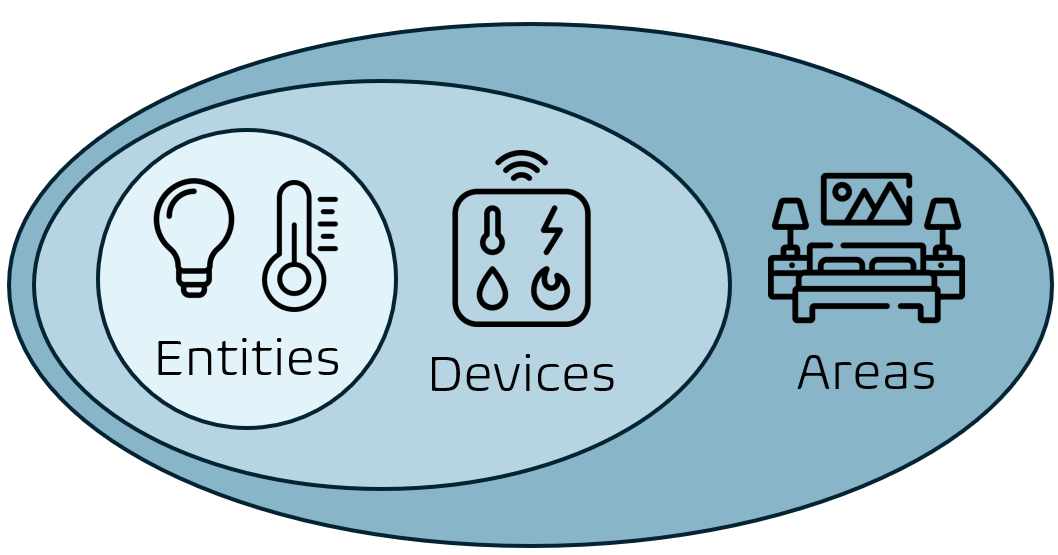
\includegraphics[width=0.8\linewidth]{images/HA_structure.png}
    \caption{The main hierarchy of HA \protect\footnotemark}
    \label{fig:ha_structure}
\end{figure}


\paragraph{Entities}
These are the lowest level possible. They represent single sensors/actuators like a temperature sensor, a lightswitch, a light, etc.
\paragraph{Devices}
These are a group of entities. It could be that a device has 1 entity (ex. a lightswitch), but it also could have multiple entities (ex. a motion sensor that is also capable of capturing the temperature).
\paragraph{Areas}
These are groups of devices that could correspond to rooms in a house. For instance, the living room could have devices like a light-switch, a motion sensor (that detects if someone is in the room), a set of speakers, etc. All of these devices could be grouped together in one area.
\paragraph{Scenes}
Scenes are used to automatically set a room to a predefined state. This could, for example, be to pre-configure the actuators of the living room to watch a movie. The user could set up a scene where, if activated, all the lights dim, the tv turns on and all the blinds in the living room close. 
\paragraph{Automations}
Automations are used to automate things. These automations consist of three things.
First a ``trigger'' needs to happen to activate the automation. This could, for example be, a motion sensor detecting movement. After the trigger, possible ``conditions'' are checked. These are additional requirements that need to be met before executing the automation, for example, ensuring someone is home. Finally ``actions'' are performed, these are the outcomes that occur after a trigger and when the conditions are met, like turning on the light in a room.
\paragraph{Scripts}
Scripts are predefined actions that are usable in automations. For example, a user may create a script to turn on all the lights in a room. This script can then be utilized in an automation that turns on the lights when someone enters the room. If the user later wants to create another automation to turn on the lights when the carport opens, they can reuse the same script. The benefit of scripts is their maintainability: if a new light is added to the room, the user only needs to update the script. Both automations will automatically use the updated script, eliminating the need to modify each automation individually.

\footnotetext{Icons by \url{https://www.flaticon.com/free-icons/pixel}} % footnote voor symbooltjes in fig:ha_structure

\subsection{Home assistant's UI}
As specified above, HA's UI has two parts. The dashboard, which is fully customizable by the user, and the automation editor, which is a pre-configured UI.
\paragraph{Dashboard}
The dashboard is the central interface where users control their smart home. It is primarily built using widgets, which can represent virtually anything the user envisions. For instance, a widget could represent a single room, containing sub-widgets to control each device within that room. Alternatively, a widget could display the entire house, allowing users to manage all devices from a single view. Users even have the option to create individual dashboards for each room if they wish. An example of a dashboard is found in Figure~\ref{fig:ha_dashboard_ex}. This dashboard is used as one of the demo's on the HA website~\cite{HA_demo}.

%While the possibilities are virtually endless, this flexibility can also pose a challenge: creating a custom dashboard from scratch might feel overwhelming for new users. To address this, HA provides support for community-built dashboards that users can adopt and expand upon as needed, making the experience more approachable and user-friendly.

\begin{figure}
    \centering
    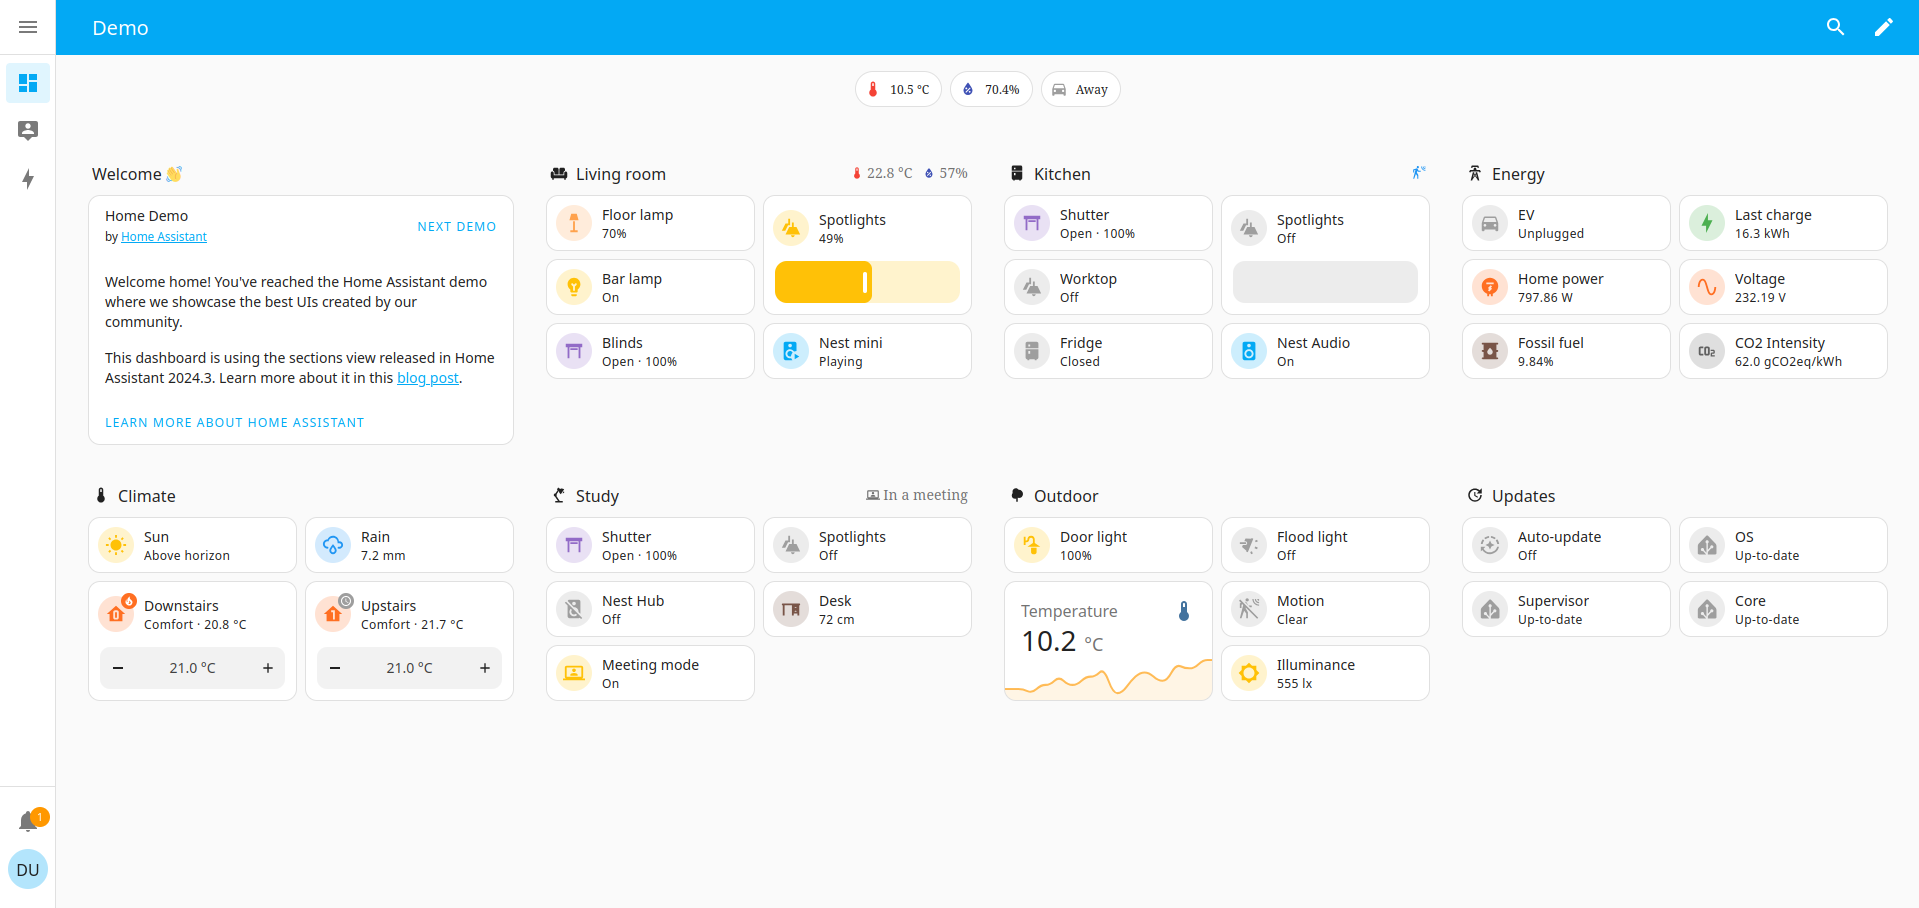
\includegraphics[width=1\linewidth]{images/HA_dashboard_ex.png}
    \caption{An example of a dashboard in HA}
    \label{fig:ha_dashboard_ex}
\end{figure}

\paragraph{Automation editor}
The automation editor is designed for creating and editing automations. It follows a fixed structure: a trigger is specified first, followed by a condition, and concluded with an action.

This consistent structure offers a key advantage: users only need to learn one framework for creating automations. However, this approach has its drawbacks. Users still need to understand how devices should be utilized within this framework, which can be challenging without prior knowledge. Additionally, by managing automations across separate user interfaces, it becomes difficult to maintain a clear overview of what each automation is designed to do.



\section{\fodot}
\label{fodot}
\fodot \footnote{\fodot is pronounced ``Eff-Oh-dot''} (aka FO-dot) is the Knowledge Representation Language used by the IDP-Z3 reasoning engine~\cite{IDPZ3ReasoningEngine}. It is an extension of first-order logic (FOL), which makes use of the following logic operators $\land, \lor, \neg, \Rightarrow, \forall, \exists$, further described in Table~\ref{tab:fodot_symbols}.

\begin{table}
    \centering
    \caption{Explanation of symbols used by \fodot}
    \label{tab:fodot_symbols}
    \begin{tabular}{|c|c|c|}
    \hline
    \fodot symbol & ASCII characters & meaning \\ \hline
    $\land$  & $\&$ & logical and   \\ \hline
    $\lor$   & $\mid$ & logical or   \\ \hline
    $\neg$   & $\sim$ & logical not   \\ \hline
    $\Rightarrow$ & $=>$ & implication   \\ \hline
    $\forall$ & $!$ & for all   \\ \hline
    $\exists$   & $?$ & for at least 1   \\ \hline
    \end{tabular}
\end{table}


The IDP-Z3 language consists of, at a minimum, a vocabulary and a theory. The vocabulary is used to describe which symbols will be used in the theory. The theory consists of rules that apply to these symbols. The structure, which is optional, describes a single, specific situation. Here is a simple example to illustrate these blocks and the basics of \fodot:

\begin{idplisting}
vocabulary V {
    type Light
    type State := {On, Off}
    
    stateOfLight: Light -> State
    brightnessLvl: Light -> Int
    isSomeoneHome: () -> Bool
}

theory T:V {
    {
       // A light is Off if the brightnesslevel is equal to 0
       !l in Light: stateOfLight(l) = Off <- brightnessLvl(l) = 0.
       
       // A light is On if the brightnesslevel is greater then 0
       !l in Light: stateOfLight(l) = On <- brightnessLvl(l) > 0.
    }
    
    // if nobody is home, then all the lights should be off
    !l in Light: ~isSomeoneHome() => stateOfLight(l) = Off.
    
    // the brightnesslvl of all the lights should be divisable by 10 and stay between 0 and 100
    !l in Light: (brightnessLvl(l) >= 0) & (brightnessLvl(l) =< 100) & (brightnessLvl(l) % 10 = 0).  
    
    // the light l should be off, if and only if nobody is home or the brightnessLvl is equal to 0
    !l in Light: stateOfLight(l) = Off <=> (~isSomeoneHome() | (brightnessLvl(l) = 0)).
}

structure S:V {
    Light := {light1, light2, light3, light4}.
    stateOfLight :> {light1 -> On, light3 -> Off}.
    brightnessLvl :> {light2 -> 60}.
}


\end{idplisting}
This \fodot description outlines the functionality of lights within a smart home. The following sections break down and explain each block in detail.

\paragraph{Vocabulary}
The lights are defined by creating a type called ``Light'' in the vocabulary. Additionally, a type called ``State'' is defined, which has two possible values: ``On'' and ``Off''. A type, in essence, represents a domain of values, in this example, for instance, a ``State'' that has 2 values: ``On'' and ``Off''. Alongside types, several functions are also defined in the vocabulary. These map one or more inputs to an output.
\begin{itemize}
    \item ``stateOfLight'': it takes a ``Light'' and maps it to a ``State''. In effect, it represents the state (``On'' or ``Off'') of a given light.
    \item ``brightnessLvl'': it takes a ``Light'' and maps it to an Integer. In effect, it represents the brightness-level of a given light.
    \item ``isSomeoneHome'': it does not take any arguments and represents a Boolean (``True'' or ``False''). This is called a proposition. It could be seen as a constant that does not change in one structure.
\end{itemize}

\paragraph{Theory}
We will now go over the four formula's in the theory.
\begin{idplisting}
!l in Light: ~isSomeoneHome() => stateOfLight(l) = Off.
\end{idplisting}
The first rule ensures that if nobody is home, the lights should be off.\\
In most cases, this can be interpreted as an ``if then'' structure. In the \fodot world, this is called an implication. If the statement on the left of the implication symbol ($\Rightarrow$) is true, then the right statement also needs to be true. However, this does not mean that if the left statement is false, the right statement can not be true.
\begin{idplisting}
!l in Light: (brightnessLvl(l) >= 0) & (brightnessLvl(l) =< 100) & (brightnessLvl(l) % 10 = 0).
\end{idplisting}
This rule ensures that the brightness level of a light remains within the range of 0 to 100. Additionally, it enforces that the brightness increments are in multiples of ten.
\begin{idplisting}
!l in Light: stateOfLight(l) = Off <=> (~isSomeoneHome() | (brightnessLvl(l) = 0)).
\end{idplisting}
The third rule ensures that the light is off if either nobody is home or the brightness level is 0, and vice versa.\\
This kind of rule uses an ``if and only if'' construct, which is more commonly referred to as an equivalence. It is used to eliminate any room for misunderstanding in an implication. If the left formula is true, the right one is too and vice versa. Consequently, if one is false, the other must be too.

\begin{idplisting}
{
   !l in Light: stateOfLight(l) = Off <- brightnessLvl(l) =< 0.
   !l in Light: stateOfLight(l) = On <- brightnessLvl(l) > 0.
}
\end{idplisting}
A light is off, then the brightness level is 0 or smaler. A light is on when the brightness level is greater then 0.\\
This last rule is a definition. It seems the same as an equivalence, but it is not. This is because using a definition explicitly indicates the intention to define the formula on the left-hand side based on the formula on the right-hand side. This sense of direction  is less apparent when using an equivalence.

\paragraph{Structure}
In the structure, a specific situation is defined. In this case, we declare that there are 4 lights and partially map some lights to states and brightness levels. The ``$:>$'' symbol stands for a partial interpretation. In this case, not all the lights are mapped. 



\section{IDP-Z3}
IDP-Z3~\cite{IDPZ3ReasoningEngine} is a reasoning engine capable of performing a variety of reasoning tasks on knowledge bases in the \fodot language. The idea is to provide knowledge (in the form of \fodot) that is used by the inference tasks of the IDP-Z3 system to produce an output. Because IDP-Z3 is build to implement the knowledge-base paradigm, it supports multiple inferences.

\subsection{The Knowledge-Base Paradigm}
The IDP-Z3 engine implements the Knowledge Base paradigm~\cite{IDPZ3KBParadigm}, in which systems store declarative domain knowledge in a knowledge base and use it to solve a variety of problems. Importantly, it states that the knowledge base should be separated from its inference tasks. This implies that the knowledge could be reused for multiple use cases within the same domain, unlike an imperative programming language where every inference would need its own separate program. Furthermore, if the KB changes, all of these programs would need to be rewritten. This is where the power of a knowledge-based system lies.\\
The multiple inference tasks are explained below using the example of the lights, shown in Section~\ref{fodot}.

\paragraph{Model expansion}
In the first place IDP-Z3 can generate models based on a given vocabulary, theory and structure. A model is a complete set of values that satisfies the theory. Figure~\ref{fig:IDP-Z3_model-generation} shows 3 possible models of the lights example. 

\begin{figure}
    \centering
    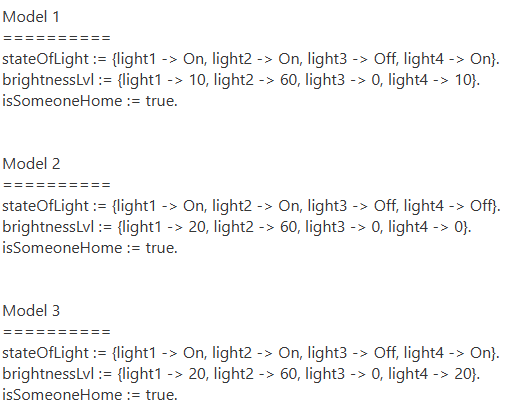
\includegraphics[width=0.8\linewidth]{images/IDP-Z3_model-generation.png}
    \caption{10 possible models in line with the provided theory and structure}
    \label{fig:IDP-Z3_model-generation}
\end{figure}

\paragraph{Propagation}
The reasoning engine can compute all the logical consequences of a certain rule. In the first implication of the theory, it is stated that if no one is home, the light needs to be in the ``Off'' state. So, if the lights are on, IDP-Z3 can infer that there must be someone home.

\paragraph{Explanation}
IDP-Z3 can provide an explanation to certain models and tell the user why one can or cannot exist. This is a task that, among other uses, is used in the Interactive Consultant UI in the online IDE, which is shown below in Figure~\ref{fig:IDP-Z3_interactive-consultant_light-example} and is further explained in Section~\ref{interactive_consultant}.

\paragraph{Optimisation}
The reasoning engine can optimize models. For example, the second rule of the theory states that the brightness-level of a light needs to be between 0 and 100 and that it is divisible by 10. It can work out that the smallest possible number of the brightness is 0. An example of this is shown in Figure~\ref{fig:IDP-Z3_interactive-consultant_optimization-example}

\paragraph{Relevance}
IDP-Z3 can figure out if there are any irrelevant symbols in the KB. Some rules of the theory are repeated below to further explain this. Rule 1 states that a light is ``Off'' either when the brightness-level of that lamp is 0 or nobody is home (and vice versa because it is an equivalence). However, this rule is irrelevant:
\begin{itemize}
    \item Rule 2 states that when nobody is home, the light should be off, making the first part of the right-hand side of the equivalence irrelevant.
    \item The definition (rule 3), states that a light is ``Off'' when the brighness-level of the light is 0, making the second part irrelevant.
\end{itemize}

\begin{idplisting}
(1) !l in Light: stateOfLight(l) = Off <=> (~isSomeoneHome() | (brightnessLvl(l) = 0)).
(2) !l in Light: ~isSomeoneHome() => stateOfLight(l) = Off.
(3) {
       !l in Light: stateOfLight(l) = Off <- brightnessLvl(l) =< 0.
       !l in Light: stateOfLight(l) = On <- brightnessLvl(l) > 0.
    }
\end{idplisting}

%\begin{itemize}
    %\item It can produce models based on the knowledge that is provided (model expansion)
    %\begin{itemize}
    %    afbeelding van de output (IDP-Z3\_model-generation.png)
    %\end{itemize}
    %\item It can understand links between types (propagation)
    % \begin{itemize}
    %     \item[] The light can be on or off if someone is home. This is defined in the first implication (first line in the theory).
    % \end{itemize}
    % \item It can explain why a sertain model can exist (explanation)
    % \begin{itemize}
    %     \item[] afbeelding van den interactive consultant (IDP\_Z3\_model-explanation.png)
    % \end{itemize}
    % \item It can optimise situations (optimisation)
    % \begin{itemize}
    %     \item[] The second rule of the theory states that the brightness-level of a lamp needs to be between 0 and 100 and that it is divisible by 10. It can work out that the smallest possible number of the brightness is 0.
    % \end{itemize}
    % \item It can check if some knowledge is redundend (relevance)
    % \begin{itemize}
    %     \item[] The last rule states that if a light is off, either the brightness-level of that lamp needs to be 0 or nobody can be home. Because of the $\Leftrightarrow$, this rule works both ways. So, if the brightness-level of a lamp is 0 or nobody is home, that light should be off. However when nobody is home, the light should already be off (the first rule of the theory). IDP-Z3 can work this out by itself.
    % \end{itemize}
%\end{itemize}

%% The output of the reasoning engine provides possible models, all of which comply with the provided theory. It also shows that the reasoning engine has assigned values to the ages of the individuals, even though these were never specified in the \fodot description. This demonstrates the power of separating the knowledge (\fodot description) from the interpretation (performed by IDP-Z3). A single knowledge base (KB) can be used for multiple purposes: it can generate models (as in this example), validate a model, or teach a user the thought process behind a certain decision.
% "The KB is ``only'' a formal representation of declarative properties of the domain. This imposes a strong requirement on the KB language (\fodot): its expressions should be interpretable as (informal) propositions about the domain, and this interpretation, its informal semantics, should be as clear, precise, and objective as possible" (Building a Knowledge Base System for an Integration of Logic Programming and Classical Logic).
% This approach contrasts strongly with declarative programming frameworks, where each operation (generation, validation, explanation, etc.) must be separately programmed. Moreover, if a change occurs, all programs must be rewritten, whereas in a system with a separated KB and interpretation, only the KB needs to be updated.

\subsection{Interactive consultant}
\label{interactive_consultant}
As said before, the Interactive Consultant~\cite{InteractiveConsultant} (IC) is a UI integrated into the online IDE of IDP-Z3, allowing users to interact with and test their constructed KB. The user can enter values, after which the IC automatically adjusts the other values, predicates, and functions so that they are in line with the KB. This can be a great tool to get insight in a KB. The usefulness is further explained using the example of the lights from Section~\ref{fodot}.

As shown in Figure~\ref{fig:IDP-Z3_interactive-consultant_light-example}, the IC explains to the user why certain behavior is implied. In this case, the KB states that a light is ``On'' if the brightness level of that light is greater than 0. So when the user sets the brightness level of ``light1'' to 40, the light should be ``On''. The ``isSomeoneHome()'' predicate also became ``True''. This is because if no one is home, all the lights should be ``Off''. This is a great showcase of how IDP-Z3 can propagate.

It can also explain to the user why a combination of values, created by the user, cannot exist, as shown in Figure~\ref{fig:IDP-Z3_interactive-consultant_error-example}. The user wanted to make the brightness level of ``light2'' 45, which is in conflict with the rule that states that the brightness level of every light must be between 0 and 100 and be divisible by 10.

The IC can also optimize some values. As shown in Figure~\ref{fig:IDP-Z3_interactive-consultant_optimization-example}, ``light1'' is minimized by pressing the button hovered over by ``light2''. The brightness level is 0, because if the light is ``Off'', its brightness level can be 0. It can not be any lower because of the rule that states that the brightness level of any light must be between 0 and 100 and be divisible by 10. ``light3'' however is turned on, so its brightness level cannot be 0. It also cannot be 1 because of the same rule that limits the brightness level.

\begin{figure}
    \centering
    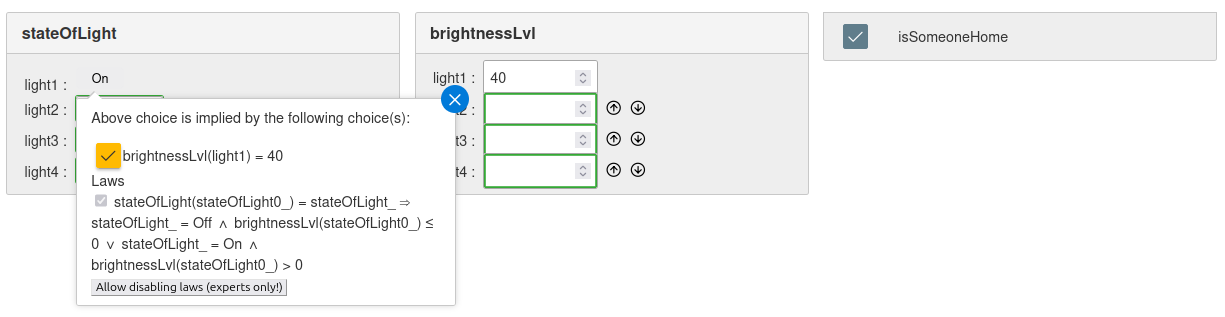
\includegraphics[width=0.8\linewidth]{images/IDP-Z3_interactive-consultant_light-example.png}
    \caption{An example off how the Interactive Consultant explains a model}
    \label{fig:IDP-Z3_interactive-consultant_light-example}
\end{figure}

\begin{figure}
    \centering
    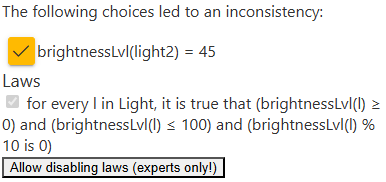
\includegraphics[width=0.4\linewidth]{images/IDP-Z3_interactive-consultant_error-example.png}
    \caption{An example of how the Interactive Consultant explains why a model can not exist}
    \label{fig:IDP-Z3_interactive-consultant_error-example}
\end{figure}

\begin{figure}
    \centering
    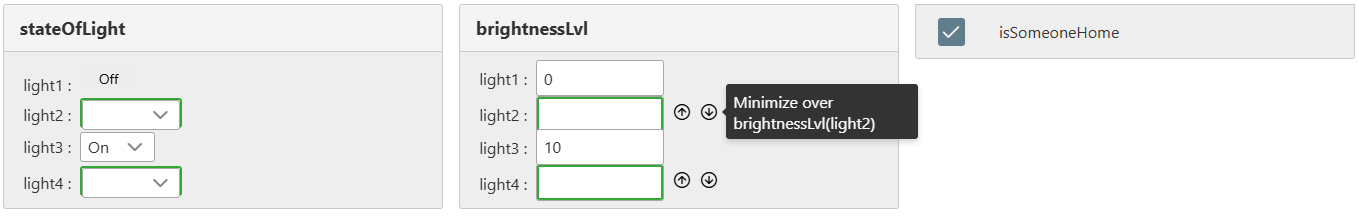
\includegraphics[width=0.8\linewidth]{images/IDP-Z3_interactive-consultant_optimization-example.png}
    \caption{An example off how the Interactive Consultant optimizes over something}
    \label{fig:IDP-Z3_interactive-consultant_optimization-example}
\end{figure}



\section{Alternatives for \fodot}
Given that \fodot can be difficult to learn and understand for non-expert users, it is useful to explore other options for more accessible interfaces. In this section, we consider alternative options in the context of home automation.

\subsection{DMN}
The Decision Model and Notation (DMN) standard~\cite{DMN} is a user-friendly notation for decision logic. It is managed by the Object Management Group (OMG), and aims to be an intuitive language that can be used by anyone involved in the modeling process. A DMN model has two main components:
\begin{itemize}
	\item Decision Requirements Diagram (DRD)
    \item Decision Tables (DT)
\end{itemize}

\paragraph{Decision Requirements Diagram}
A DRD is a graph-like structure that represents which decision should be made. It includes input fields (rounded boxes) that provide the system with data needed for making decisions. The squared boxes denote decisions.
\paragraph{Decision Tables}
A DT describes a decision. It defines the output based on a set of input variables. It requires these variables to be fully enumerated, meaning that all possible combinations must be covered. It also needs to capture the necessary and sufficient conditions. These conditions ensure that all criteria must be met to produce a particular output, and when one condition is met, it leads directly to the corresponding output.\\
The example shown in Figure~\ref{fig:DT} represents the definition of the lights example, its \fodot representation can be found below. It states that a light is ``On'' if the brightness level is greater then 0 and that it is ``Off'' if the brightness level is 0. Important to note is that all DTs can be represented by a \fodot definition, but not all \fodot definitions can be represented by a DT. Similarly, implications cannot be represented in a DT. 

\begin{idplisting}
{
   !l in Light: stateOfLight(l) = Off <- brightnessLvl(l) =< 0.
   !l in Light: stateOfLight(l) = On <- brightnessLvl(l) > 0.
}
\end{idplisting}

\begin{figure}
    \centering
    \dmntable{Define state of light}{U}{brightnessLevel}{stateOfLight}{
    $\geq 0$, on,
    $\leq 0$, off
}
    \caption{An example of a Decision Table using the example of the lights}
    \label{fig:DT}
\end{figure}


\paragraph{ Pros and cons}
The main advantage of using DMN is its clarity and user-friendliness. The user does not need any programming knowledge to model with it effectively. However, a significant drawback is its limited capabilities. When the user attempts to describe more complex situations, it can quickly become very unreadable, so much so that some solutions to those situations fail to meet DMN's readability goals.
 
\paragraph{cDMN}
cDMN~\cite{cDMN} is an extension of DMN that addresses the shortcomings of standard DMN by introducing constraint modeling, quantification, types, and functions. Although this makes cDMN more complex, it is far more readable than a complex, standard DMN. By adding these things, an implication is possible, as shown in Figure~\ref{fig:cDMNTable}. If no one is home, the light should be off. The \fodot code that represents this table is shown below.
 
\begin{idplisting}
!l in Light: ~isSomeoneHome() => stateOfLight(l) = Off.
\end{idplisting}

\begin{figure}
    \centering
    \dmntable{Disable lights if nobody's home}{E*}{isSomeoneHome}{stateOfLight}{
        No, off
    }
    \caption{An example of a cDMN table using an implication of the example of the lights}
    \label{fig:cDMNTable}
\end{figure}
 
\subsection{CNL}
\label{CNL}
A Controlled Natural Language~\cite{CNL} (CNL) is a subset of a natural language (e.g. English) that is strictly defined. This allows it to be understood by both a computer and a human. This is useful because the domain experts do not need an expert on the language. According to~\cite{CNLAttemptoControlledEnglish}, a CNL consists of two parts:
 \begin{itemize}
 	\item A subset of a language used as ``syntax'' 
     \item A parsing engine so the computer can understand the language
 \end{itemize}
 IDP-Z3 has its own CNL, which is used in its Interactive Consultant. This thesis will use this as an example.

\paragraph{The IDP-Z3 CNL}
The example of the lights, written in CNL and shown below, is used as an example. The CNL is likely to make it much more readable to the average person. Another way in which the online IDE makes use of this CNL is in its Interactive Consultant. In the screenshot shown in Figure~\ref{fig:IDP-Z3_interactive-consultant_light-example} the explanation is useful and helps the user understand what is going on, but it still requires some understanding of FO symbols, which is not ideal.
The example below shows the CNL as a replacement for \fodot. While it is more readable, there is still a clear reference to the \fodot language. It feels unintuitive to say ``for all l in Light'', instead of ``for every Light l''. While the second phrasing is clearer for humans, the order change makes it so the IDP-Z3 system can not understand it.

\begin{idplisting}
vocabulary V {
    type Light
    type State is {On, Off}
    stateOfLight: Light -> State
    brightnessLvl: Light -> Int
    isSomeoneHome: () -> Bool
}
theory T:V {
    {
        for all l in Light : stateOfLight(l) = Off if brightnessLvl(l) =< 0 .
        for all l in Light : stateOfLight(l) = On if brightnessLvl(l) > 0 .
    }
    for all l in Light : not isSomeoneHome() are sufficient conditions for stateOfLight(l) is Off .
    for all l in Light : (brightnessLvl(l) is greater than 0) & (brightnessLvl(l) is less than 100) & (brightnessLvl(l) % 10 is 0) .
    for all l in Light : (stateOfLight(l) is Off) is the same as (not isSomeoneHome() or (brightnessLvl(l) is 0)) .
}
structure S:V {
    Light := {light1, light2, light3, light4} .
}
\end{idplisting}

\paragraph{Pros and cons}
A CNL allows the user to create easy-to-read code because it uses a subset of a known language, removing the need of a technical expert on the used language. However, it is not the easiest to write due to its strictness with the ordering of words, which can introduce confusion. Two structures that seem the same to us humans, may be interpreted differently by the computer. The limited set of words available in a CNL can also pose challenges. While the user might prefer to write in natural, unrestricted text as they are accustomed to, the computer is unable to interpret such input. This challenge, known as the writability problem~\cite{CNL}, highlights the difficulty of creating a language that remains readable without introducing ambiguity, so the computer can still understand it.
These restrictions can lead to an unintended consequence: writing in a CNL may become more challenging than learning the actual language it is meant to simplify. Users end up learning not only the syntax but also the boundaries of what is and is not possible within the CNL, which can be frustrating and counterproductive.

\subsection{Blocks-based editor}
A blocks-based editor is a user-friendly way to write software using blocks. This allows the user to avoid memorizing syntax, as the blocks are provided and visually indicate what is possible and what is not, eliminating the need to understand complex syntax rules. In other words, syntax errors are non-existent, allowing the user to fully focus on what the application should do, rather than how to write it in a certain language. However, the workspace can become disorganized as projects grow larger.

A well-known example of a blocks-based programming enviroment is Scratch~\cite{scratch}, a blocks-based interface in JavaScript. It allows users to create programs in a visual workspace, while processing the blocks into runnable JavaScript code. Scratch is a code editor designed for children, ensuring that it needs to be understandable even for the youngest users. In Figure~\ref{fig:scratch} an example of a workspace is shown.

\begin{figure}
    \centering
    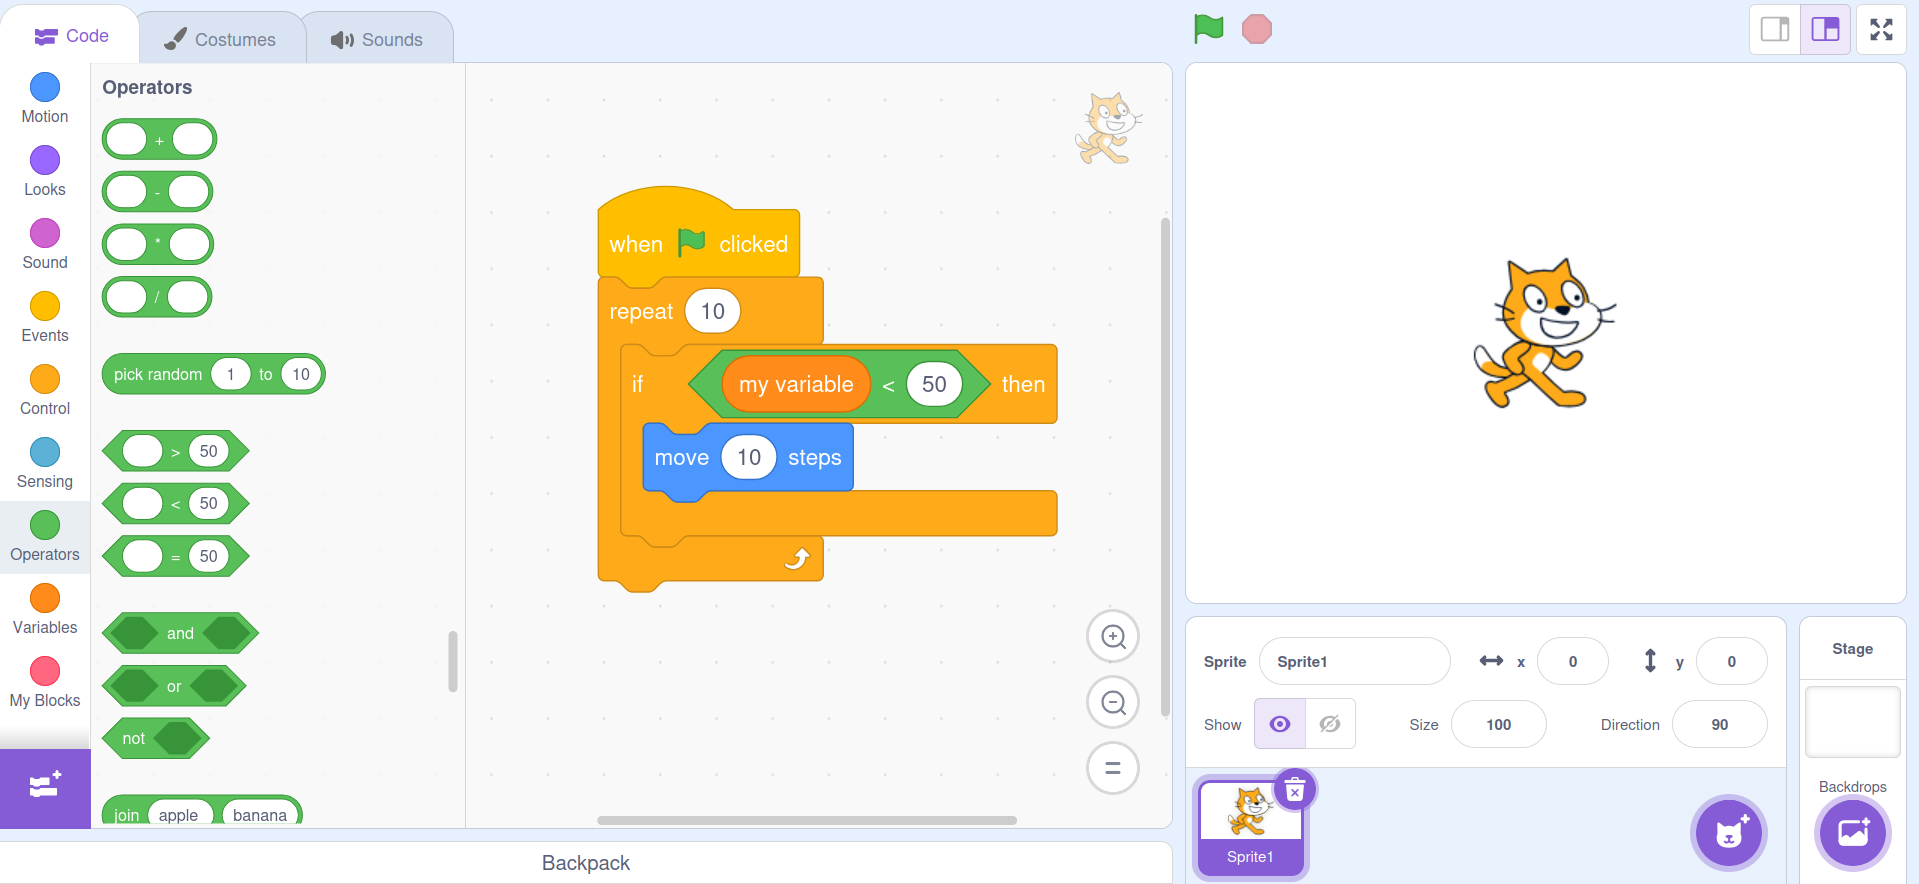
\includegraphics[width=1\linewidth]{images/block-based_scratch.png}
    \caption{An example of the scratch UI}
    \label{fig:scratch}
\end{figure}

\paragraph{\fodot blocks-based editor}
There already exists a blocks-based editor for \fodot~\cite{IDPStructuredBlockbasedEditor}. It uses Blockly~\cite{Blockly}, an extendable blocks-based editor developed by Google. It has two components:
\begin{itemize}
	\item A workspace where blocks can be placed
	\item A generator where blocks are translated to a textual representation (in this case \fodot)
\end{itemize}
An example of this editor is shown in~\ref{fig:blockly_IDP_example}. This is, however, too complex for what is needed for IoT in home automation. Still, it provides a good baseline to start from.

\begin{figure}
    \centering
    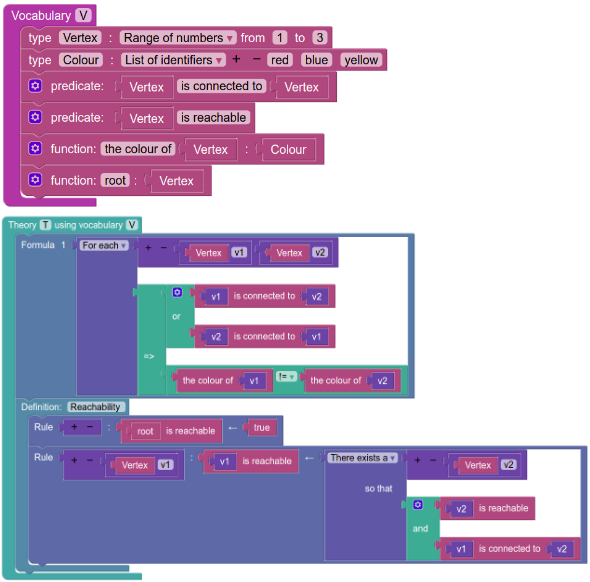
\includegraphics[width=0.8\linewidth]{images/blockly_IDP_example.png}
    \caption{An example of a Blockly editor for \fodot}
    \label{fig:blockly_IDP_example}
\end{figure}

\paragraph{Pros and cons}
A blocks-based editor is very clear and easy in how to use it. The user can not make syntax errors, because they can see what blocks fit each other and which do not. This implies that no expert of the language (or blocks) is needed to create a working project. However, by making it all visual, it can get messy quite quickly. For bigger projects, that need more complex functionality, the workspace can get very unorganised and difficult to navigate. There are some ways to try and fix this, for example by creating a new block with combined funtionality which is described in its own workspace. 

An overview of the meaningful pro's and con's of all the discussed user-friendly interfaces can be found in Table~\ref{tab:user-friendly_comparison}.

\begin{table}
    \centering
    \caption{Comparison of user-friendly interfaces \fodot}
    \label{tab:user-friendly_comparison}
    \begin{tabular}{|c|c|c|c|}
    \hline
    User-friendly interface & Graphical interface & Low code & Sufficiently expressive \\ \hline
    DMN & x & x &   \\ \hline
    IDP-Z3 CNL &  &  & x  \\ \hline
    Blocks-based editor & x & x & x \\ \hline
    \end{tabular}
\end{table}

\section{State of the art}
In this chapter we will describe previous works on logical reasoning and home automation. More specificially an example of other ways to implement knowledge bases. Why the use of YAML files for home automation configuration is not ideal for people without a background in programming. Why knowledge based systems work for home automation and why blocks-based editors are a good user-friendly option for non-experts.  

\subsection{IntelliDomo}
IntelliDomo~\cite{SOTA_OntologyBased} is an ontology-based interface for HA. It uses an ontology (OntoDomo) to represent the KB, production rules (written in SWRL (Semantic Web Rule Language)) to describe the system, and an inference engine (Jess) to make decisions.

The KB is represented in OWL files (Ontology Web Language), which are created by the system using existing ontologies. This is convenient when an appropriate ontology already exists; however, if there is none, the user must understand OWL to create their own. IntelliDomo uses SWRL in combination with a custom-made UI for rule construction. This ensures that users cannot make syntax errors, as all possible options are predefined. However, the UI still has the SWRL syntax in it, so it still requires the user to know SWRL even tough they do not need to write any. Since SWRL is not the most intuitive language for writing rules for a non-expert, it can be challenging to follow the logic it describes.

This paper demonstrates that a knowledge-based approach to home automation works, but it is important to note that their approach is not the most user-friendly one. This is however very important when it comes to automating your home.

When considering how AI can help both with user-friendliness and how the user describes their home automation system, according to \cite{SOTA_KnowledgeBasedAIInHomeAutomation}, knowledge-based AI fits into this perfectly. It is easier for non-experts to create a knowledge-based home automation system than it is to create a traditional sequentially programmed system because a KB system is much more flexible. However, it still requires the user to modify the rules of the KB when circumstances change. While this can also be automated using AI, that will not be discussed here.

\subsection{Issues with the current automation configuration}
Home automation configuration often relies on YAML files for defining a home's setup, which is how HA manages configurations behind the scenes. If certain automations cannot be configured through the HA UI, users must modify these YAML files themselves. However, YAML is not the most user-friendly language for non-experts, making it challenging for users to implement these more complex automations. Fortunately, HA has an active community that often helps less experienced users navigate these difficulties.

Despite this support, the community still struggles to address certain challenges. As highlighted in~\cite{SOTA_AutomationConfigurationSmarthome}, users face three primary issues when modeling their homes in YAML: debugging (68\%), implementation (27\%), and optimization (5\%). The paper evaluates six validation tools, including the HA IDE, and reports that while these tools demonstrate high precision -- meaning errors identified are likely genuine (75\%-94\%) -- they suffer from very low recall, identifying only 9-11 bugs out of 129.

This indicates that while validation tools exist, they are not very effective in practice. Robust validation is essential for users, as they are likely to encounter bugs or problems that cannot be resolved through an IDE. This often forces them to edit YAML files directly, which is not ideal. Even worse, if mistakes are made in the YAML files, identifying and correcting them becomes nearly impossible without better tools or an active community. When designing a user-friendly application, validation should be kept in consideration.

\subsection{Smart Block}
\label{SmartBlock}
SmartBlock~\cite{SOTA_SmartBlock} is a user-friendly blocks-based interface for the SmartThings IoT platform. They built their editor using Blockly~\cite{Blockly}, a JavaScript framework for creating blocks-based editors. It is also worth mentioning that they added tools to check for inconsistencies and mistakes made by the user.

They conducted a user study with 33 participants from diverse backgrounds (including IT). First, the participants were asked to model a rule to get familiar with the editor. 81\% of them responded positively or neutrally to the ease of use. After this introduction, the participants were tasked with modeling three progressively more challenging rules. Over time, they got better at this, which was shown by how much faster they were able to complete the tasks. Interestingly, the difference in performance between non-IT and IT participants was not that big, which further shows how user-friendly the editor is.

Another test required the participants to identify some errors in a given SmartApp. This proved to be more difficult without assistance, as the debugging tools lacked any semantic error correction. This highlights why having a tool to correct mistakes during the modeling process is so important.

This paper proves that a blocks-based editor is a viable option for home automation. It shows that such an editor is user-friendly and accessible to people without an IT background. It also confirms the importance of tools that can help with semantic errors.


% \chapter{Plans for next semester}
% In the next part, I will focus on developing a user-friendly, blocks-based editor for IDP-Z3. In the next chapter, I will now elaborate on the reasoning behind this choice and outline the approach we plan to take for its development at this stage.
% 
% \section{Blocks-based editor for IDP-Z3}
% In this section, we will discuss why we chose a blocks-based editor and how we see the implementation.
% \subsection{User-friendly interface}
% We are choosing to implement a blocks-based editor. The primary reason for this decision is the need to learn the, for non-experts, difficult \fodot-syntax and the advantages that a blocks-based editor offers to address this challenges. The \fodot language, along with its syntax, is not particularly readable for non-experts. In contrast, a blocks-based editor eliminates the need for syntax entirely, as it visually indicates what can and cannot be combined. This approach makes it impossible for users to make syntax errors.
% 
% Another significant benefit of a blocks-based editor is that it does not feel like traditional coding. Instead, it feels like the user is piecing together a puzzle that happens to produce code, which makes the process more intuitive and approachable. This is not always the case with other user-friendly editors. For example, while a CNL does not feel like coding either, its strict structure can make it feel unnatural, as discussed in Section~\ref{CNL} regarding the writability problem. A DMN is also visual, but lacks the expressiveness required for our modeling purposes. It is insufficient to describe only definitions when other useful symbols are needed but cannot be represented in DMN. Although cDMN resolves these limitations, it introduces additional complexity, making it less accessible for non-expert users.
% 
% Blocks-based editors have already proven to be highly user-friendly. A prominent example is Scratch, which designed for children, who typically have no prior understanding of programming. Scratch’s success highlights the effectiveness of blocks-based interfaces in simplifying programming concepts. Furthermore, as discussed in Section~\ref{SmartBlock}, existing literature frequently references blocks-based editors compared to other user-friendly alternatives. The study mentioned in that section, involving 33 participants, further supports the usability and effectiveness of blocks-based editors.
% 
% A crutual aspect of the editor we plan to make is validation of the rules created by the user. Others~\cite{SOTA_AutomationConfigurationSmarthome} have already proven that this is crutial for the user-friendlyness of such an editor. We plan to let the users interact with their ruleset through the Interactive Consultant of IDP-Z3, as this is already quite clear.
% 
% \subsection{Structure and implementation}
% We intend to use Blockly, a blocks-based editor written in JavaScript. Blockly allows developers to create custom blocks with specific functionality. We will leverage this capability to design an interface that bridges the gap between a user-friendly editor and the \fodot language. The editor will generate a ``.idp'' file, which can serve as a KB to be processed and reasoned over by IDP-Z3. We also aim to incorporate an interface similar to the Interactive Consultant discussed in Section~\ref{interactive_consultant}. This addition will allow users to interact with their constructed KB, enabling them to test and verify whether the behavior aligns with their intentions. To ensure seamless communication and data transfer between systems, we will utilize Python. 
% 
% \subsection{Verification}
% We plan to conduct user testing with a group of individuals who have no background in home automation or programming. By asking them to model specific examples, we can effectively evaluate whether our goal of creating a user-friendly interface has been achieved.
% 
% \subsection{Planning}
% My planning for the second semester is shown in Figure~\ref{fig:planning}.
% \begin{figure}
%     \centering
%     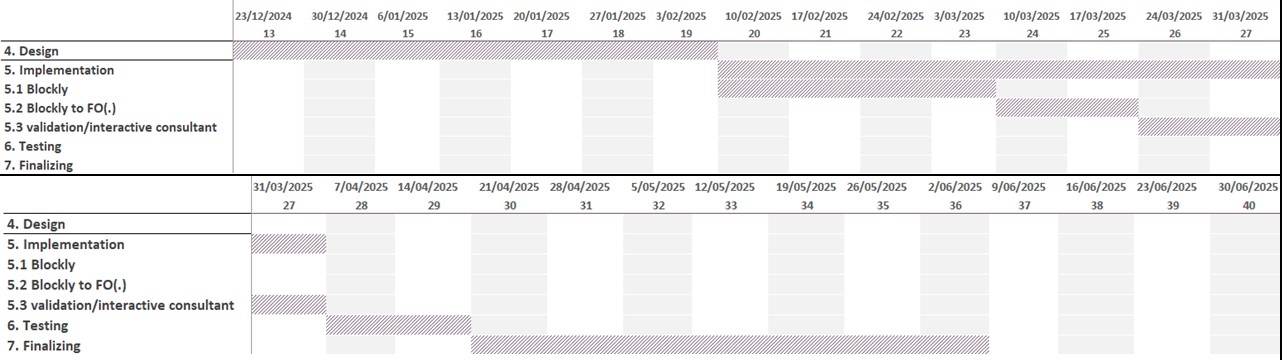
\includegraphics[angle=90, width=0.4\linewidth]{images/planning.png}
%     \caption{Planning for the second semester}
%     \label{fig:planning}
% \end{figure}

% \chapter{Home automation description}
% In this chapter we will discuss what a user could want in their home automation system. It is important to understand what the user would want to do with their home automation system. We will need to bring these things into the \fodot description, so the user can model their home in a way that is useful to them.% 
% \section{Devices}% 
% The user will want to configure their devices in an intuitive way, which does not require them to understand how the devices are configured in the application. Each device has possible states it can be in, for example a lightswitch can be ``On'' or ``Off''. The user could configure these states themselves, but most devices already have a standard set of states. Home assistant also uses the standard states of%  the devices to configure them in their UI. This is great, since the user does not need to figure out the possible states of a device themselves. However, to implement this in an editor, we will need to read out the states of a lot of device-types, which will not % be done in this editor.
% \section{Areas}% 
% The user will want to configure their devices in a way that matches the layout of their home, this way they can create rules that apply to devices in a room, which can be very handy. The user can for example create a rule that turns off all the lights in the bedroom when nobody is in set bedroom. Since the user will set up the areas matching their house, it will create a new way that the user can understand % what they are doing. This is a great way to make the user feel more comfortable with the system.
% 
\chapter{An \fodot description for home automation}
In this chapter we will discuss different ways to implement a home automation system in \fodot. However, before we can do that, we need to figure out what the user expects from their home automation system. How we can achive a meaningful and logic description that offers a lot of flexibility, while keeping it simple enough so it is doable using ``simple'' blocks. We will discuss the advantages and disadvantages of some implementation and which of these we will use going forward.
\begin{figure}
    \centering
    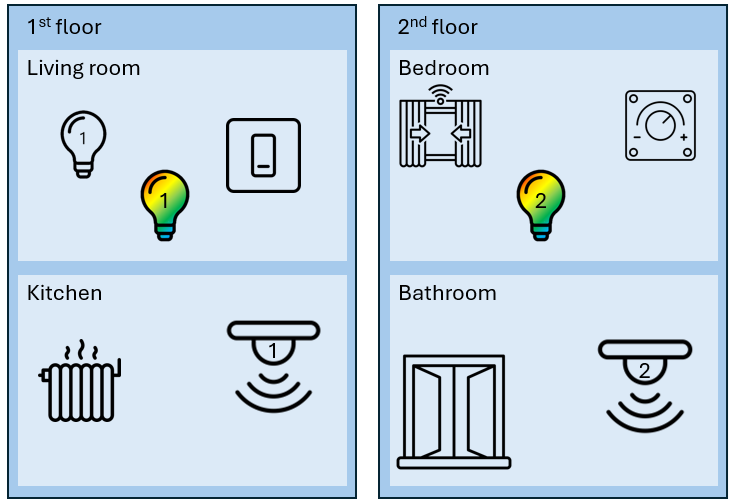
\includegraphics[width=0.8\linewidth]{images/fodot-structure_example.png}
    \caption{An example of a home automation system used to explain the different \fodot implementations}
    \label{fig:fodot-structure_example}
\end{figure}

\section{Home automation description}
\paragraph{Devices}
The user will want to configure their devices in an intuitive way, which does not require them to understand how the devices are configured in the application. Each device has possible states it can be in, for example a lightswitch can be ``On'' or ``Off''. The user could configure these states themselves, but most devices already have a standard set of states. Home assistant also uses the standard states of the devices to configure them in their UI. This is great, since the user does not need to figure out the possible states of a device themselves. However, to implement this in an editor, we will need to read out the states of a lot of device-types, which will not be done in this editor.
\paragraph{Areas}
The user will want to configure their devices in a way that matches the layout of their home, this way they can create rules that apply to devices in a room, which can be very handy. The user can for example create a rule that turns off all the lights in the bedroom when nobody is in set bedroom. Since the user will set up the areas matching their house, it will create a new way that the user can understand what they are doing. This is a great way to make the user feel more comfortable with the system.
\paragraph{Rules}
It is important to think about what the user would want to configure and what rules they would want to create. Below are some examples of rules the user could want to create increasing in complexity the further down the list.
\begin{itemize}
    \item Turn on a light when a lightswitch is turned on.
    \item Set the brightness of a light to 50 when the lightswitch is turned on.
    \item Set an RGB light to the colour yellow when the lightswitch is turned on.
    \item Turn on light0 and light1 when the lightswitch is turned on.
    \item Turn on all the lights in the living room when the lightswitch is turned on.
    \item Turn off all the lights in the living room and turn on all the lights in the kitchen when the motionsensor in the kitchen is triggered.
    \item Turn off all the lights on the first floor when a motion sensor on the second floor is triggered.
\end{itemize}

\section{Vocabulary}
The vocabulary is an important part of the \fodot specification as it defines the possibilities and limits for the rest of the specification. There are lots of different aproaches possible, where each needs to be effective with the idea of ease of use and effectiveness in a real-world application.

The first vocabulary is one that is easy to create from blocks due to the way devices are represented. Each device has its own constant, which is linked to an area. So when creating a possible model, a device could be ``light1 -> livingRoom''. The problem with this way of representing the devices is that there is no way to group the devices. A rule that states that all the devices in the living room should be turned off is not possible, but is something the user would defenitly want. The states of these devices are represented through a type that defines all possible states for that device. In combination with this, there is a function that represents what state the device is in. 

An other shortcomming of this vocabulary is the inability to represent relations between areas. This is because the vocabulary does not allow to group devices, as stated earlier, as well as the inability to group areas. This is also something the user would want to have since it could be a way to structure their home in the application which makes it feel familiar.
\begin{idplisting}
vocabulary V {
    type Area := {living_room, kitchen, floor_1, floor_2, house}
    light1: -> Area
    type stateOfLight <: Int
    stateOfLight1: -> stateOfLight
}
\end{idplisting}
The second vocabulary improves on both of these shortcomings by defining a type ``Device,'' under which all specific instances of devices fall. This allows for the creation of rules that apply to all devices, specific devices, and areas. The only slight drawback of this vocabulary is that IDP-Z3 does not provide much assistance if anything is wrongly defined. It would be preferable if IDP-Z3 could offer more support in preventing user mistakes.
\begin{idplisting}
vocabulary V {
    type Device
    type Area
    deviceIsInArea: Device -> Area
    deviceIsBell: Device -> Bool
    type BellState := {ringing, off}
    bellState : Device -> BellState 
}
\end{idplisting}
This is where the third and final vocabulary comes in. Instead of focusing on the devices themselves, the focus now lies on the states of the devices and their grouping. By using subtypes, different instances of devices can be created according to their state. For example, a motion sensor is binary (motion detected or no motion detected), but a light switch is also binary (on or off), so these can be grouped together. This vocabulary does not differ much from the previous one, in the sence that if all devices have different states, it will result in the same behaviour, but it opens up possibilities for more complex rules. This approach is slightly more challenging to construct using blocks, but the possibilities this vocabulary offers outweigh this drawback.
\begin{idplisting}
vocabulary V {
type Device
type BinaryDevice <: Device
type BinaryState := {on, off}
binaryDeviceState: BinaryDevice -> BinaryState    
}
\end{idplisting}
Having experimented with all tree of the possibilities, we have decided to go with the second vocabulary. It offers the user the flexibility they want, while keeping it simple enough so they understand what is going on and being able to model it with simple blocks. The first vocabulary is a bit too simple and does not offer the user the flexibility they want, it is however very easy to create blocks for it. The thrid vocabulary is complexer but it does not offer more functionality then the second one, so it is not worth the extra work to make the conversion from blocks to IDP-Z3 more complex.

An important note to make is the fact that these vocabularies limit the user in what they can do in the theory, this is how the \fodot language is desinged, so it is important that the vocabulary does not limit the posibilities. However, since this is not just the \fodot description, some functionality (that is not possible in \fodot) can be implemented in the blockly backend. This is further explored in ....

\printbibliography
\end{document}